\documentclass[letter,11pt]{article}
%\documentclass[letter,twoside,11pt]{article}

\usepackage[spanish,es-nodecimaldot]{babel}
\usepackage[utf8]{inputenc}

\usepackage{lmodern}
\usepackage[T1]{fontenc}
\usepackage{textcomp}

\usepackage{graphicx}
\usepackage{pstricks}

\usepackage{anysize}
\marginsize{3cm}{2cm}{2cm}{3cm}

\usepackage{amsmath}
\usepackage{array}

\usepackage{fancyhdr}
\usepackage{lastpage}
\pagestyle{fancy}
\fancyhf{}
\fancyhead[LE,RO]{Laboratorio de Física Básica I}
\fancyfoot[CO,CE]{\thepage\ de \pageref{LastPage}}

\special{papersize=215.9mm,279.4mm}

\usepackage[
    pdfauthor={Carlos Eduardo Caballero Burgoa},%
    pdftitle={Laboratorio de Física Básica I},%
    pdfsubject={Mediciones indirectas y propagación de errores},%
    colorlinks,%
    citecolor=black,%
    filecolor=black,%
    linkcolor=black,%
    urlcolor=black,
    breaklinks]{hyperref}
\usepackage{breakurl}

\newcommand{\blankpage}{
\newpage
\thispagestyle{empty}
\mbox{}
\newpage
}

\renewcommand{\arraystretch}{1.2}

\begin{document}

\begin{titlepage}
\begin{center}
{\Large UNIVERSIDAD MAYOR DE SAN SIMÓN}\\
\vspace*{0.15cm}
{\large FACULTAD DE CIENCIAS Y TECNOLOGÍA}\\
\vspace*{0.10cm}
DEPARTAMENTO DE FÍSICA\\
\vspace*{3.0cm}
{\Large \textbf{LABORATORIO DE FÍSICA BÁSICA I}}\\
\vspace*{0.3cm}
{\Large \textbf{PRACTICA No. 2}}\\
\vspace*{3.5cm}
{\Large \textbf{MEDICIONES INDIRECTAS Y PROPAGACIÓN DE ERRORES}}\\
\end{center}

\vspace*{6.9cm}
\leftskip=7.95cm
\noindent
\textbf{Estudiante:}\\
Caballero Burgoa, Carlos Eduardo.\\
\newline
\textbf{Docente:}\\
Msc. Guzmán Saavedra, Rocio.\\
\newline
\textbf{Grupo:} N5.\\
\textbf{Fecha de realización:} 23 de Octubre del 2020.\\
\textbf{Fecha de entrega:} 27 de Octubre del 2020.\\

\end{titlepage}

\blankpage

\section{Objetivo}
Que el estudiante se familiarice con la representación de las medidas
indirectas.

\section{Marco teórico}
Las mediciones indirectas son mediciones donde no es posible obtener un valor
directamente con el instrumento de medición. Para determinar el valor de la
medición es necesaria una función matemática que relacione las magnitudes.

Para la determinación del error de las mediciones indirectas, se utiliza el
método de propagación de errores, es decir, la propagación o efecto que
producen los errores de las mediciones directas al error de la función.

Consideremos el calculo del valor de una magnitud $y$, que es función de una
serie de magnitudes $x_1, x_2, \dots, x_n$, cuyos valores se pueden obtener de
una manera directa en el laboratorio, es decir que:

\begin{equation}
\label{eq:f}
    y = f(x_1,x_2,\dots,x_n)
\end{equation}

donde $x_i$, son los resultados de mediciones directas, ellas son conocidas como
variables independientes:

\begin{equation}x_1 = (\bar{x}_1 \pm e_1)[u],\end{equation}
\begin{equation}x_2 = (\bar{x}_2 \pm e_2)[u],\end{equation}
\begin{equation}x_n = (\bar{x}_n \pm e_n)[u],\end{equation}

La mejor estimación de $y$ se obtiene sustituyendo en la expresión \ref{eq:f}
los valores obtenidos de $\bar{x}_i$:

\begin{equation}
    \bar{y} = f(\bar{x}_1,\bar{x}_2,\dots,\bar{x}_n)
\end{equation}

Para la estimación del error de $\bar{y}$ se utiliza la siguiente formula:

\begin{equation}
    e_y = \sqrt{\sum_{i=1}^{n}
    \left(\left|\frac{\partial{f}}{\partial{x_i}}\right|_{\bar{x}_i}
    e_i\right)^2}
\end{equation}

finalmente el resultado de la medición indirecta es:

\begin{equation}
    y = (\bar{y} \pm e_y)[u], E\%
\end{equation}

\section{Materiales}
\begin{itemize}
\item Calibrador \emph{Vernier} (precision 0.05[mm]).
\item Calibrador \emph{Vernier} (precision 0.1[mm]).
\item Tornillo micrométrico (precision 0.01[mm]).
\item Regla de 15 cm (precision 1[mm]).
\end{itemize}

\section{Procedimiento}
A continuación se describen los procedimientos experimentales de medición que se
llevarán a cabo.

\subsection{Calculo del área del circulo}
\begin{itemize}
\item Dado el circulo de la figura \ref{circulo}, calcular la formula del
área en función de su diámetro.
\item Calcular el valor del área utilizando la formula hallada.
\item Hallar la derivada parcial de la función con respecto al diámetro.
\item Calcular el error estimado según el criterio pitagórico.
\end{itemize}

\begin{figure}
\centering
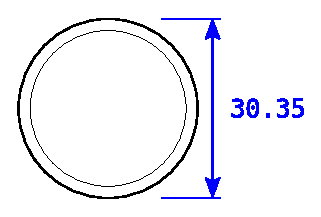
\includegraphics[width=0.25\textwidth]{eps/02_01.circulo.eps}
\caption{Datos del circulo}
\label{circulo}
\end{figure}

\subsection{Calculo del volumen del perno}
\begin{itemize}
\item Dado el perno de la figura \ref{perno}, calcular la formula del
volumen en función de sus parámetros.
\item Calcular el valor del volumen utilizando la formula hallada.
\item Hallar las derivadas parciales de la función con respecto a sus
parámetros.
\item Calcular el error estimado según el criterio pitagórico.
\end{itemize}

\begin{figure}
\centering
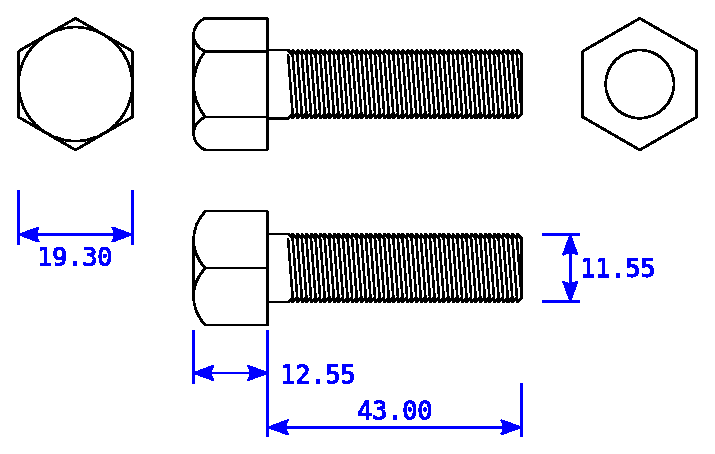
\includegraphics[width=0.58\textwidth]{eps/02_02.perno.eps}
\caption{Datos del perno}
\label{perno}
\end{figure}

\subsection{Calculo del área de una pieza}
\begin{itemize}
\item Dada la pieza de la figura \ref{pieza}, calcular la formula del
área en función de sus parámetros.
\item Calcular el valor del área utilizando la formula hallada.
\item Hallar las derivadas parciales de la función con respecto a sus
parámetros.
\item Calcular el error estimado según el criterio pitagórico.
\end{itemize}

\begin{figure}
\centering
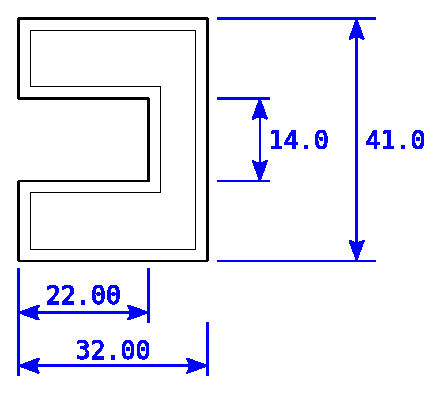
\includegraphics[width=0.35\textwidth]{eps/02_03.pieza.eps}
\caption{Datos de la pieza}
\label{pieza}
\end{figure}

\subsection{Calculo del área de una caja}
\begin{itemize}
\item Dada la caja de la figura \ref{caja}, calcular la formula del
área en función de su base y su altura.
\item Calcular el valor del área utilizando la formula hallada.
\item Hallar las derivadas parciales de la función con respecto a sus
parámetros.
\item Calcular el error estimado según el criterio pitagórico.
\end{itemize}

\begin{figure}
\centering
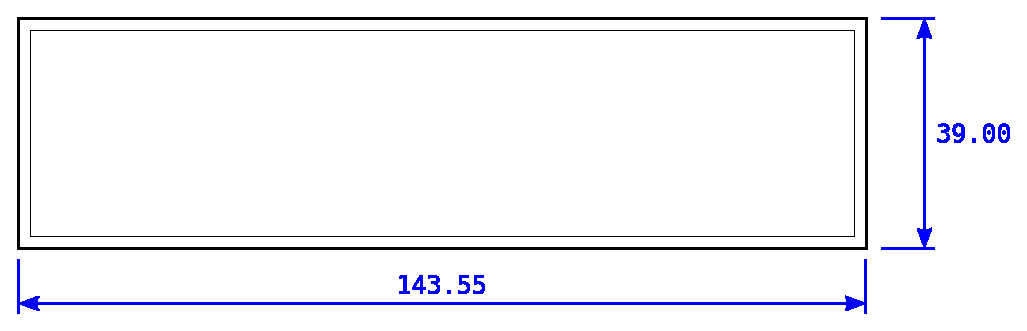
\includegraphics[width=0.85\textwidth]{eps/02_04.caja.eps}
\caption{Datos de la caja}
\label{caja}
\end{figure}

\subsection{Calculo del volumen del capacitor}
\begin{itemize}
\item Dado el capacitor de la figura \ref{capacitor}, calcular la formula del
volumen en función de sus parámetros.
\item Calcular el valor del volumen utilizando la formula hallada.
\item Hallar las derivadas parciales de la función con respecto a sus
parámetros.
\item Calcular el error estimado según el criterio pitagórico.
\end{itemize}

\begin{figure}
\centering
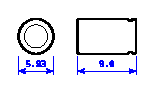
\includegraphics[width=0.32\textwidth]{eps/02_05.capacitor.eps}
\caption{Datos del capacitor}
\label{capacitor}
\end{figure}

\subsection{Calculo del volumen del tornillo}
\begin{itemize}
\item Dado el tornillo de la figura \ref{tornillo}, calcular la formula del
volumen en función de sus parámetros.
\item Calcular el valor del volumen utilizando la formula hallada.
\item Hallar las derivadas parciales de la función con respecto a sus
parámetros.
\item Calcular el error estimado según el criterio pitagórico.
\end{itemize}

\begin{figure}
\centering
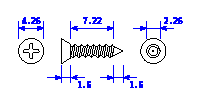
\includegraphics[width=0.45\textwidth]{eps/02_06.tornillo.eps}
\caption{Datos del tornillo}
\label{tornillo}
\end{figure}

\subsection{Calculo del volumen de la esfera}
\begin{itemize}
\item Dada la esfera de la figura \ref{esfera}, calcular la formula del
volumen en función de su diámetro.
\item Calcular el valor del volumen utilizando la formula hallada.
\item Hallar la derivada parcial de la función con respecto a su diámetro.
\item Calcular el error estimado según el criterio pitagórico.
\end{itemize}

\begin{figure}
\centering
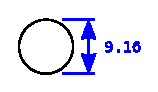
\includegraphics[width=0.20\textwidth]{eps/02_07.esfera.eps}
\caption{Datos de la esfera}
\label{esfera}
\end{figure}

\subsection{Calculo del volumen de la chapa de puerta}
\begin{itemize}
\item Dada la chapa de puerta que se muestra en la imagen \ref{fotografia},
cuyas medidas se presentan en la figura \ref{chapa}, calcular la formula del
volumen en función de sus parámetros.
\item Calcular el valor del volumen utilizando la formula hallada.
\item Hallar las derivadas parciales de la función con respecto a sus
parámetros.
\item Calcular el error estimado según el criterio pitagórico.
\end{itemize}

\begin{figure}
\centering
\includegraphics[width=0.85\textwidth]{eps/02.chapa.eps}
\caption{Chapa de puerta a calcular}
\label{fotografia}
\end{figure}

\begin{figure}
\centering
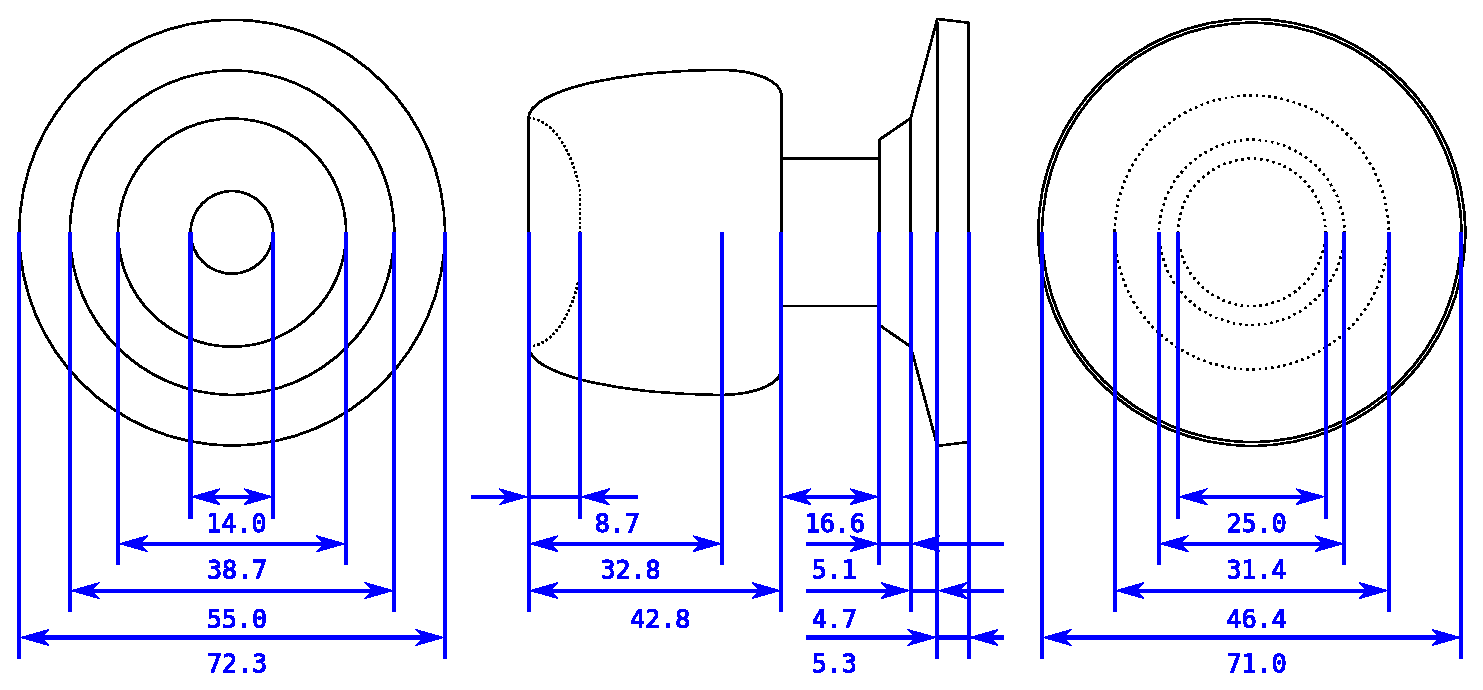
\includegraphics[width=1.00\textwidth]{eps/02_08.chapa.eps}
\caption{Datos de la chapa}
\label{chapa}
\end{figure}

\section{Tablas de datos y resultados}

\subsection{Calculo del área del circulo}
\begin{center}
\begin{tabular}{|c|>{\centering}m{5.0cm}<{\centering}|}
\hline
\multicolumn{2}{|c|}{\textbf{Medidas directas del circulo}}
\tabularnewline \hline
Diametro ($d$) & $30.35 \pm 0.05 [mm]; 0.16\%$ \tabularnewline \hline
\end{tabular}
\end{center}

Dada la ecuación para el calculo del area de un circulo en función de su
diámetro:

\begin{equation}
    A = \pi r^2 = \frac{\pi d^2}{4}
\end{equation}

Calculando el valor representativo:

\begin{equation}
    A = \frac{(3.1415)(30.35)^2}{4} = 723.45
\end{equation}

La derivada parcial es:

\begin{equation}
    \frac{\partial{A}}{\partial{d}} = \frac{\pi d}{2}
\end{equation}

Siendo el error de la medición:

\begin{equation}
    e_A = \frac{\pi d}{2} e_d
\end{equation}

Calculando el error representativo:

\begin{equation}
    e_A = \frac{(3.1415)(30.35)}{2}(0.05) = 2.38
\end{equation}

\begin{center}
\begin{tabular}{|c|>{\centering}m{5.0cm}<{\centering}|}
\hline
\multicolumn{2}{|c|}{\textbf{Resultado}}
\tabularnewline \hline
Area ($A$) & $723.45 \pm 2.38 [mm^2]; 0.33\%$ \tabularnewline \hline
\end{tabular}
\end{center}

\subsection{Calculo del volumen del perno}
\begin{center}
\begin{tabular}{|c|>{\centering}m{5.0cm}<{\centering}|}
\hline
\multicolumn{2}{|c|}{\textbf{Medidas directas del perno}}
\tabularnewline \hline
Diametro de la circunferencia inscrita ($d_i$) & $19.30 \pm 0.05 [mm]; 0.26\%$
\tabularnewline \hline
                 Longitud de la cabeza ($l_c$) & $12.55 \pm 0.05 [mm]; 0.40\%$
\tabularnewline \hline
                  Longitud del vastago ($l_v$) & $43.00 \pm 0.05 [mm]; 0.12\%$
\tabularnewline \hline
                      Diametro externo ($d_e$) & $11.55 \pm 0.05 [mm]; 0.43\%$
\tabularnewline \hline
\end{tabular}
\end{center}

\subsection{Calculo del área de una pieza}
\begin{center}
\begin{tabular}{|c|>{\centering}m{5.0cm}<{\centering}|}
\hline
\multicolumn{2}{|c|}{\textbf{Medidas directas de la pieza}}
\tabularnewline \hline
  Base externa ($b_e$) & $32.00 \pm 0.05 [mm]; 0.16\%$ \tabularnewline \hline
  Base interna ($b_i$) & $22.00 \pm 0.05 [mm]; 0.23\%$ \tabularnewline \hline
Altura externa ($h_e$) & $41    \pm 1    [mm]; 2.44\%$ \tabularnewline \hline
Altura interna ($h_i$) & $14    \pm 1    [mm]; 7.14\%$ \tabularnewline \hline
\end{tabular}
\end{center}

\subsection{Calculo del área de una caja}
\begin{center}
\begin{tabular}{|c|>{\centering}m{5.0cm}<{\centering}|}
\hline
\multicolumn{2}{|c|}{\textbf{Medidas directas de la caja}}
\tabularnewline \hline
  Base ($b$) & $143.55 \pm 0.05 [mm]; 0.03\%$ \tabularnewline \hline
Altura ($h$) & $ 39    \pm 1    [mm]; 2.56\%$ \tabularnewline \hline
\end{tabular}
\end{center}

\subsection{Calculo del volumen del capacitor}
\begin{center}
\begin{tabular}{|c|>{\centering}m{5.0cm}<{\centering}|}
\hline
\multicolumn{2}{|c|}{\textbf{Medidas directas del capacitor}}
\tabularnewline \hline
Diametro ($d$) & $5.93 \pm 0.01 [mm];  0.17\%$ \tabularnewline \hline
  Altura ($h$) & $9    \pm 1    [mm]; 11.11\%$ \tabularnewline \hline
\end{tabular}
\end{center}

Dada la ecuación para el calculo del volumen de un cilindro en función de su
altura y el diámetro de su base:

\begin{equation}
    V = \pi r^2 H = \frac{\pi D^2 H}{4}
\end{equation}

Las derivadas parciales son:

\begin{equation}
    \frac{\partial{V}}{\partial{D}} = \frac{\pi H D}{2}
\end{equation}
\begin{equation}
    \frac{\partial{V}}{\partial{H}} = \frac{\pi D^2}{4}
\end{equation}

Siendo el error de la medición:

\begin{equation}
    e_V = \sqrt{
        \left(\frac{\pi H D}{2}\right)^2 {e_D}^2 +
        \left(\frac{\pi D^2}{4}\right)^2 {e_H}^2
    }
\end{equation}

\subsection{Calculo del volumen del tornillo}
\begin{center}
\begin{tabular}{|c|>{\centering}m{5.0cm}<{\centering}|}
\hline
\multicolumn{2}{|c|}{\textbf{Medidas directas del tornillo}}
\tabularnewline \hline
Diametro de la cabeza ($d_h$) & $4.26 \pm 0.01 [mm]; 0.23\%$
\tabularnewline \hline
Longitud de la cabeza ($l_h$) & $1.60 \pm 0.01 [mm]; 0.62\%$
\tabularnewline \hline
  Longitud del cuerpo ($l_b$) & $7.22 \pm 0.01 [mm]; 0.14\%$
\tabularnewline \hline
 Longitud de la punta ($l_t$) & $1.60 \pm 0.01 [mm]; 0.62\%$
\tabularnewline \hline
     Diametro externo ($d_e$) & $2.26 \pm 0.01 [mm]; 0.44\%$
\tabularnewline \hline
\end{tabular}
\end{center}

\subsection{Calculo del volumen de la esfera}
\begin{center}
\begin{tabular}{|c|>{\centering}m{5.0cm}<{\centering}|}
\hline
\multicolumn{2}{|c|}{\textbf{Medidas directas de la esfera}}
\tabularnewline \hline
Diametro de la esfera ($d$) & $9.16 \pm 0.01 [mm]; 0.11\%$
\tabularnewline \hline
\end{tabular}
\end{center}

Dada la ecuación para el calculo del volumen de una esfera en función de su
diámetro:

\begin{equation}
    V = \frac{4}{3} \pi r^3 = \frac{\pi D^3}{6}
\end{equation}

La derivada parcial es:

\begin{equation}
    \frac{\partial{V}}{\partial{D}} = \frac{\pi D^2}{2}
\end{equation}

Siendo el error de la medición:

\begin{equation}
    e_V = \frac{\pi \bar{D}^2}{2} e_D
\end{equation}

\subsection{Calculo del volumen de la chapa de puerta}
\begin{center}
\begin{tabular}{|c|>{\centering}m{5.0cm}<{\centering}|}
\hline
\multicolumn{2}{|c|}{\textbf{Medidas directas de la chapa}}
\tabularnewline \hline
         Diametro cilindro ($d_1$) & $14.0 \pm 0.1 [mm]; 0.71\%$
\tabularnewline \hline
      Diametro minimo pomo ($d_2$) & $38.7 \pm 0.1 [mm]; 0.26\%$
\tabularnewline \hline
      Diametro maximo pomo ($d_3$) & $55.0 \pm 0.1 [mm]; 0.18\%$
\tabularnewline \hline
    Diametro maximo roseta ($d_4$) & $72.3 \pm 0.1 [mm]; 0.14\%$
\tabularnewline \hline
           Diametro cuello ($d_5$) & $25.0 \pm 0.1 [mm]; 0.40\%$
\tabularnewline \hline
    Diametro minimo roseta ($d_6$) & $31.4 \pm 0.1 [mm]; 0.32\%$
\tabularnewline \hline
Diametro intermedio roseta ($d_7$) & $46.4 \pm 0.1 [mm]; 0.22\%$
\tabularnewline \hline
     Diametro borde roseta ($d_8$) & $71.0 \pm 0.1 [mm]; 0.14\%$
\tabularnewline \hline
          Profundidad pomo ($l_1$) & $ 8.7 \pm 0.1 [mm]; 1.15\%$
\tabularnewline \hline
     Longitud barriga pomo ($l_2$) & $32.8 \pm 0.1 [mm]; 0.30\%$
\tabularnewline \hline
             Longitud pomo ($l_3$) & $42.8 \pm 0.1 [mm]; 0.23\%$
\tabularnewline \hline
           Longitud cuello ($l_4$) & $16.6 \pm 0.1 [mm]; 0.60\%$
\tabularnewline \hline
      Grosor cuello roseta ($l_5$) & $ 5.1 \pm 0.1 [mm]; 1.96\%$
\tabularnewline \hline
  Grosor intermedio roseta ($l_6$) & $ 4.7 \pm 0.1 [mm]; 2.13\%$
\tabularnewline \hline
        Grosor base roseta ($l_7$) & $ 5.3 \pm 0.1 [mm]; 1.89\%$
\tabularnewline \hline
\end{tabular}
\end{center}

\section{Conclusiones}
Puede notarse que las mediciones indirectas agrandan el error que las mediciones
directas ya tienen, se ha considerado mejorar la precisión de los instrumentos
para objetos que son pequeños como en este caso.

\subsection{Resumen de mediciones}
A continuación se resumen las medidas obtenidas:

\begin{center}
\begin{tabular}{|c|>{\centering}m{5.0cm}<{\centering}|}
\hline
\textbf{Circulo} & \tabularnewline \hline
\textbf{Perno} & \tabularnewline \hline
\textbf{Pieza} & \tabularnewline \hline
\textbf{Caja} & \tabularnewline \hline
\textbf{Capacitor} & \tabularnewline \hline
\textbf{Tornillo} & \tabularnewline \hline
\textbf{Esfera} & \tabularnewline \hline
\textbf{Chapa} & \tabularnewline \hline
\end{tabular}\\
\end{center}

\section{Referencias bibliográficas}
\begin{itemize}
\item Errores de medición y su propagación \\
http://www.tplaboratorioquimico.com/2008/08/errores-de-medicion-y-su-propagacion.html
\item Tratamiento y propagación de errores \\
http://www.lawebdefisica.com/apuntsfis/errores/
\item Informe de propagación de errores \\
http://www.slideshare.net/cdloor/informe-de-propagacion-de-errores-laboratorio-de-fisica-c
\item Guía práctica para la realización de la medida y el calculo de errores \\
http://bacterio.uc3m.es/docencia/laboratorio/guiones\_esp/errores/guiondeerrores.pdf
\end{itemize}

\end{document}
